\documentclass[a4paper,12pt]{article}

\usepackage[utf8]{inputenc}
\usepackage{amsmath, amssymb}
\usepackage{graphicx}
\usepackage{geometry}
\usepackage{hyperref}
\usepackage{setspace}
\usepackage{fancyhdr}
\usepackage{float}
\usepackage{lipsum}
\usepackage{listings}
\usepackage{xcolor}
\usepackage{xcolor-material}

\geometry{margin=1in}

\pagestyle{fancy}
\fancyhf{}
\fancyhead[L]{Laporan Final Sistem Tertanam}
\fancyhead[R]{\thepage}

\lstdefinestyle{mystyle}{
    backgroundcolor=\color{white},
    commentstyle=\color{green},
    keywordstyle=\color{magenta},
    numberstyle=\tiny\color{gray},
    stringstyle=\color{purple},
    basicstyle=\ttfamily\footnotesize,
    breakatwhitespace=false,
    breaklines=true,
    frame=single,
    captionpos=b,
    keepspaces=true,
    numbers=none,
    numbersep=10pt,
    showspaces=false,
    showstringspaces=false,
    showtabs=false,
    tabsize=2,
}

\lstset{style=mystyle}

\begin{document}
\begin{titlepage}
    \centering
    \vspace*{1cm}
    {\Large \textbf{Laporan Final \textit{Game PingPong} pada \textit{Dotmatrix Display}}}
    \vfill
    \vspace{2cm}

    
\includegraphics[width=0.4\textwidth]{./images/logo.png}
    \vfill

    \vspace{1cm}
    \begin{onehalfspace}
    \textbf{Dosen Pengampu}\\
    Eko Pramunanto, S.T. M.T.

    \vspace{1cm}

    \textbf{Disusun Oleh:}\\
    Muhammad Haekal Muhyidin Al-Araby\\
    5024221004\\
    Sistem Tertanam - A
    \end{onehalfspace}

    \vfill

    \textbf{DEPARTEMEN TEKNIK KOMPUTER\\
    FAKULTAS TEKNOLOGI ELEKTRO DAN INFORMATIKA CERDAS\\
    INSTITUT TEKNOLOGI SEPULUH NOPEMBER\\2024}
\end{titlepage}


\section{Komponen}
\begin{enumerate}
    \item ESP32\\
    ESP32 sebagai mikrokontroller yang digunakan untuk mengendalikan dotmatrix
    melalui program yang telah dipasang atau flash.
    \item MAX7219 8x32 LED Dot Matrix Display Module\\
    Modul terdiri dari 4 buah dot matrix dan IC MAX7219 yang digunakan untuk sebagai
    penghubung antara ESP32 dan display dotmatrix. Bertindak sebagai decoder dan selector.
    \item PCB\\
    Sebagai tempat untuk merangkai barang yang ada dan menyambungkannya.
    \item Pin Header Female\\
    Untuk menghubungkan ESP32 dengan PCB.
    \item Pin Header Male Siku\\
    Menghubungkan display ke PCB
    \item Push Button\\untuk input smash
    \item Slide Potentiometer\\input gerakan player
\end{enumerate}

\section{Desain Sistem}
\subsection{Rangkaian Skematik}
\begin{figure}[H]
    \centering
    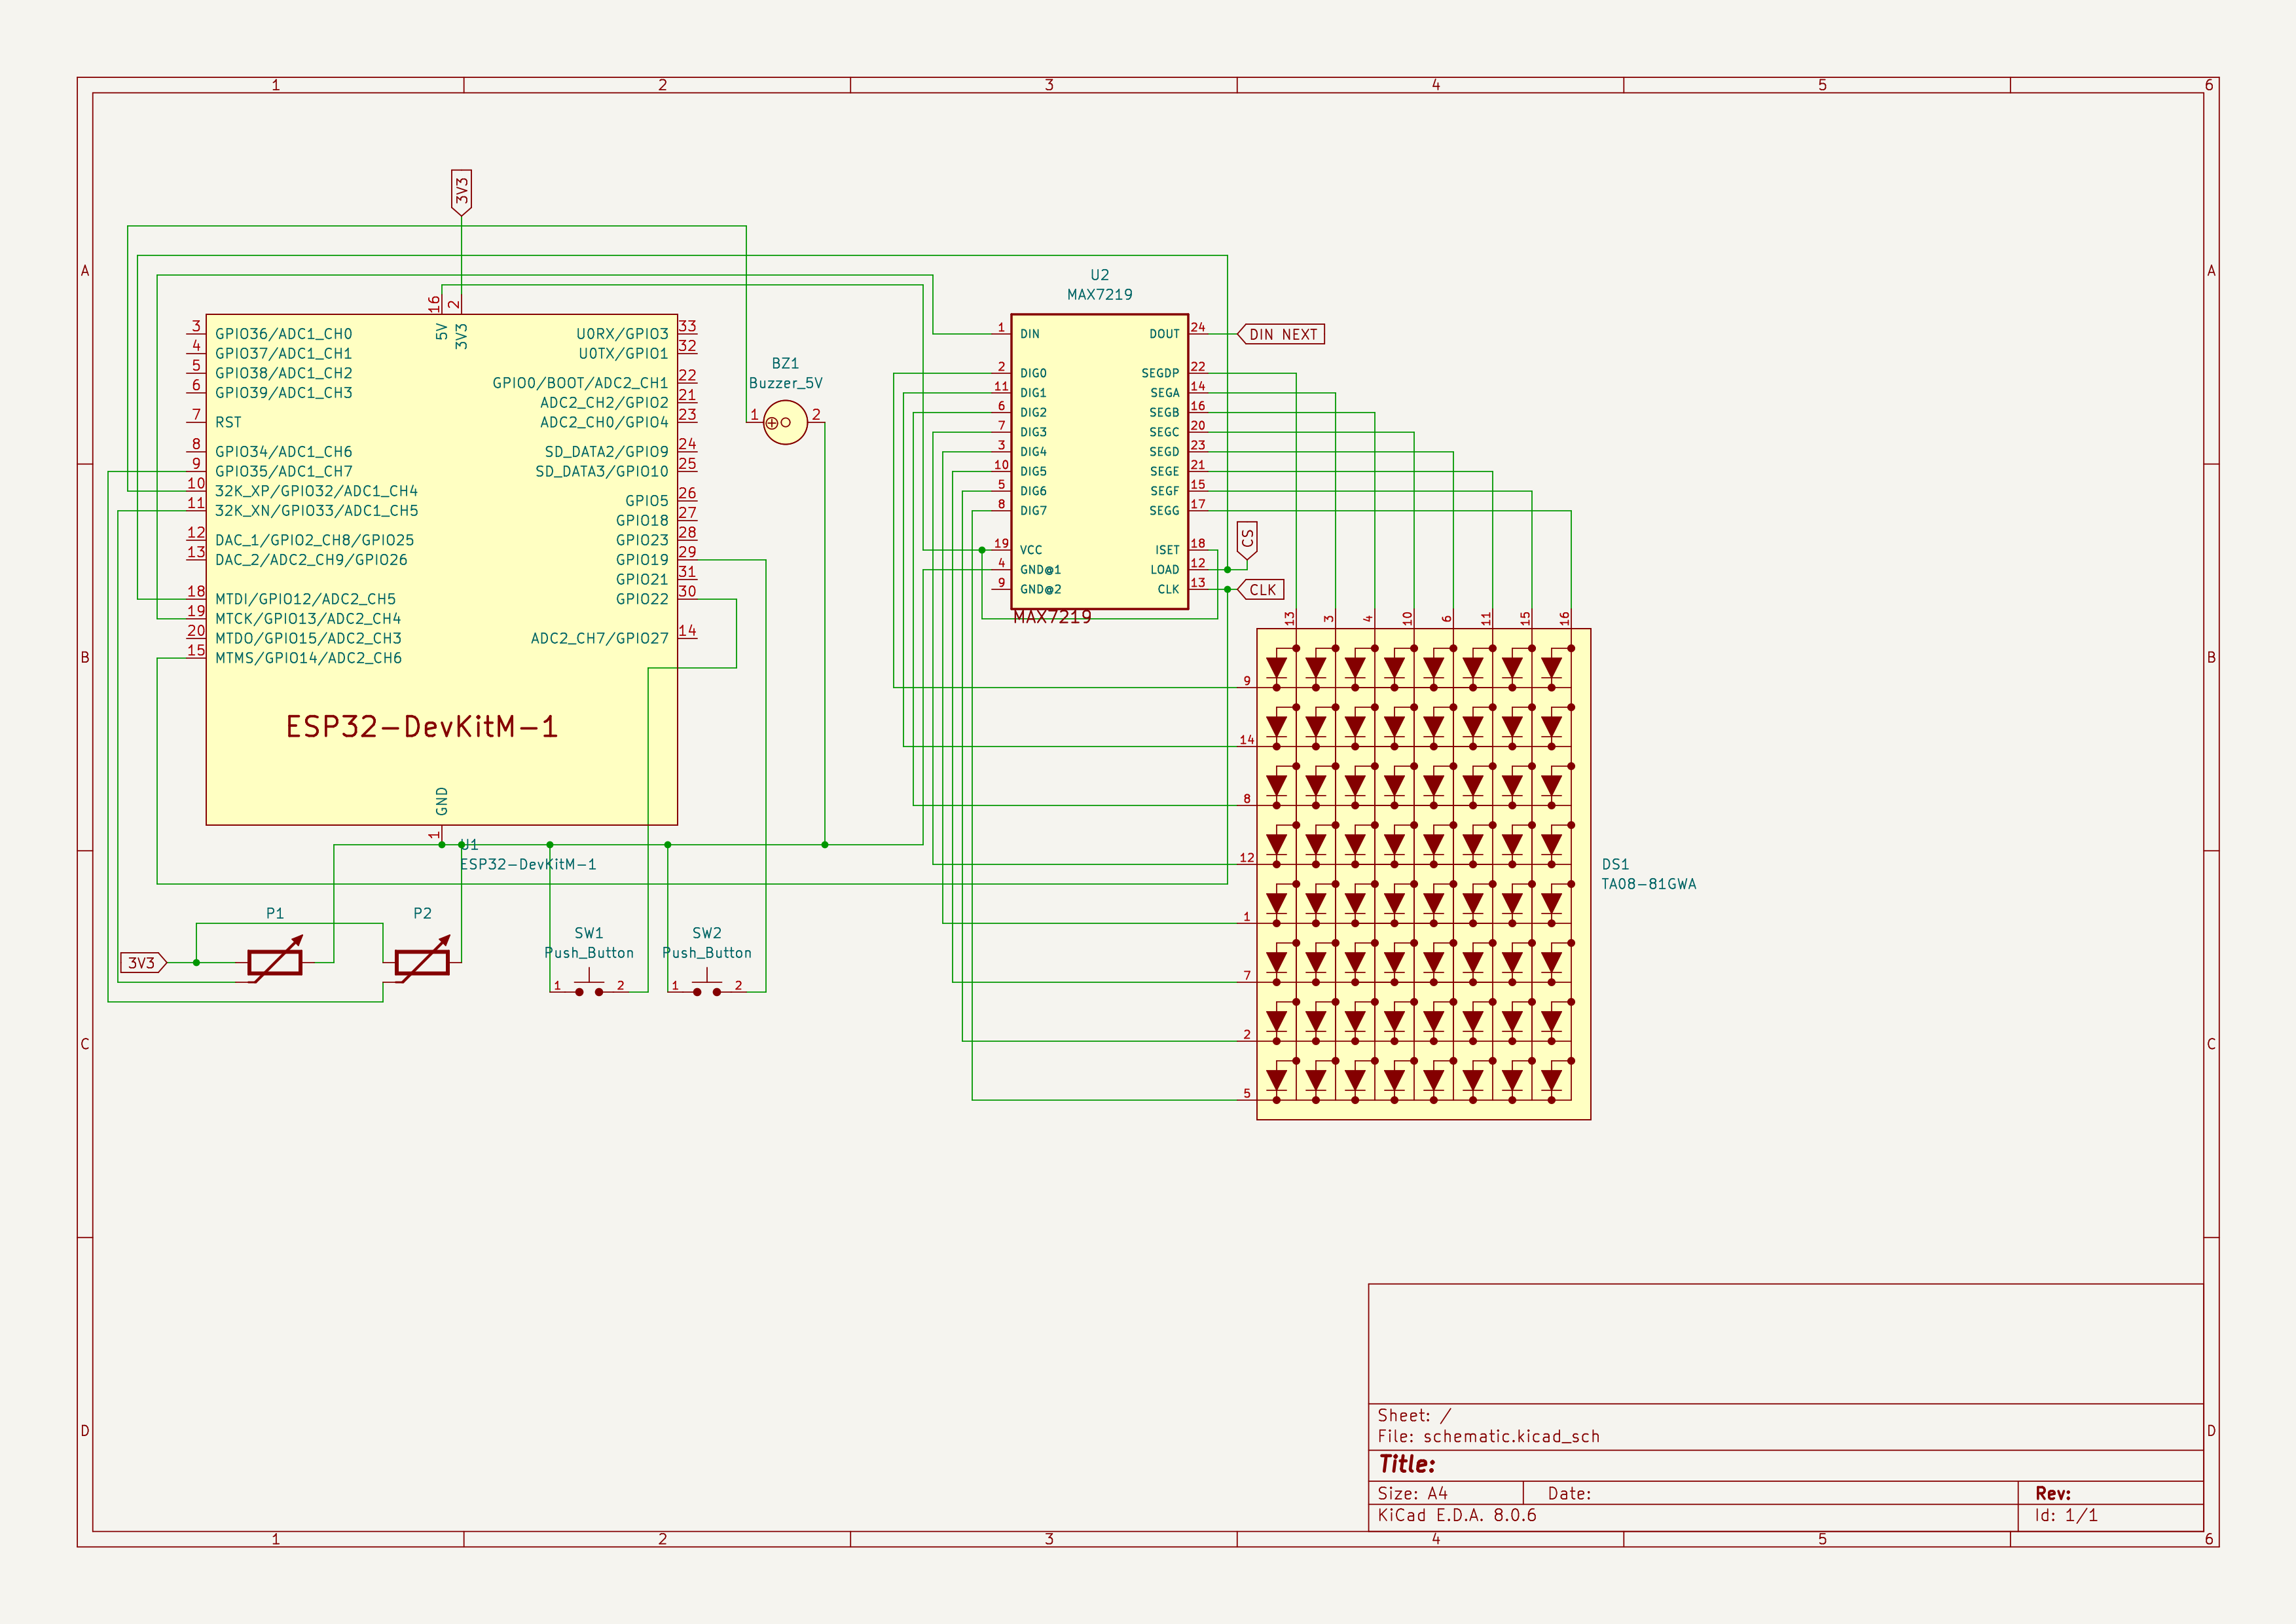
\includegraphics[width=1\textwidth]{images/schematic.png}
    \label{fig:schematic}
    \caption{Schematic}
\end{figure}
Rangkaian menggunakan ESP32 yang terhubung pada IC MAX7219 dimana CS
terhubung pada pin D12, DIN pada D13 dan clock pada D14
terdapat 4 IC MAX7219 yang saling terhubung secara seri. Lalu push button dihubungkan dengan
ground dan GPIO dan potentiometer dihubungkan ke ground, vcc, dan GPIO.
\subsection{Desain Game}
\begin{figure}[h!]
    \centering
    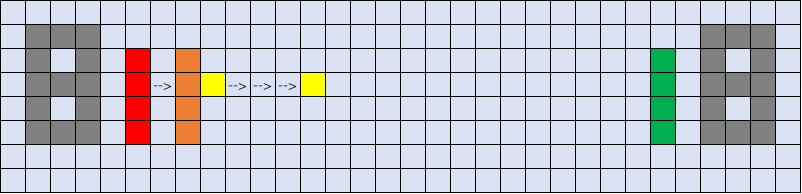
\includegraphics[width=1\textwidth]{images/desain_game.png}
    \label{fig:desaingame}
    \caption{Desain Game}
\end{figure}
\begin{enumerate}
    \item Game memiliki 2 player yang dapat digerakkan dengan slide potentiometer
    \item Bola akan memantul saat menabrak pembatas ataupun player
    \item Bola memantul secara diagonal dengan kecepatan konstan
    \item Bila player smash dan mengenai bola, bola akan bergerak lurus dan lebih cepat
    \item Bila bola melewati player maka player lainnya akan mendapatkan skor
    \item Player yang kebobolan akan mendapatkan bola dan dapat menggerakkannya
        dan menekan tombol smash untuk service.
    \item Game akan berakhir bila salah satu pemain mencapai skor 11 dan selisih 2 poin.
    \item Game akan berakhir imbang ketika kedua pemain mencapai 15 poin
\end{enumerate}

\subsection{Program}
\subsubsection{Menampilkan}
Untuk menampilkan ke dotmatrix dapat digunakan 2 library MD\_Parola dan MD\_MAX72xx. Dimana MD\_Parola dapat
menampilkan huruf namun kurang dalam kontrol sehingga akan kesulitan untuk menampilkan Game. Sehingga MD\_Parola hanya akan digunakan
saat menampilkan string. Sedangkan saat ingin menampilkan karakter akan menggunakan MD\_MAX72xx yang memberikan raw control pada
dotmatrix display. Untuk itu akan dibuat sebuah fungsi yang menerima input berbentuk array 8*32 untuk ditampilkan pada dotmatrix. Berikutnya
akan disebut frame. Lalu tiap objek akan diupdate dengan diletakan pada frame tersebut. Sesuai dengan posisi.

\subsubsection{Input}
Input didapatkan dengan mengambil nilai analogRead pada potentiometer dan digitalRead pada button smash.
\subsection{Source Code}
Berisi program utama yang mengatur main loop.
\lstinputlisting[language=C++, caption={main.cpp}]{../src/main.cpp}
Program di bawah mengendalikan device dotmatrix menggunakan library Parola dan MDMAX
\lstinputlisting[language=C++, caption={device.hpp}]{../include/device.hpp}
\lstinputlisting[language=C++, caption={device.cpp}]{../src/device.cpp}
Program di bawah menampilkan untuk menampilkan Intro
\lstinputlisting[language=C++, caption={animation.hpp}]{../include/animation.hpp}
\lstinputlisting[language=C++, caption={animation.cpp}]{../src/animation.cpp}
Program di bawah Berisi class vector2 untuk memudahkan posisi game object
\lstinputlisting[language=C++, caption={vector2.hpp}]{../include/vector2.hpp}
\lstinputlisting[language=C++, caption={vector2.cpp}]{../src/vector2.cpp}
Program di bawah berfungsi mendapatkan input player dan mengupdate state player
\lstinputlisting[language=C++, caption={player.hpp}]{../include/player.hpp}
\lstinputlisting[language=C++, caption={player.cpp}]{../src/player.cpp}
Program di bawah untuk mengupdate state bola
\lstinputlisting[language=C++, caption={ball.hpp}]{../include/ball.hpp}
\lstinputlisting[language=C++, caption={ball.cpp}]{../src/ball.cpp}
Program di bawah untuk menyalakan buzzer
\lstinputlisting[language=C++, caption={buzzer.hpp}]{../include/buzzer.hpp}
\lstinputlisting[language=C++, caption={buzzer.cpp}]{../src/buzzer.cpp}
Program di bawah untuk memunculkan skor
\lstinputlisting[language=C++, caption={score.hpp}]{../include/score.hpp}
\lstinputlisting[language=C++, caption={score.cpp}]{../src/score.cpp}
Program di bawah berisi Global Variabel yang digunakan seluruh program
\lstinputlisting[language=C++, caption={global.hpp}]{../include/global.hpp}
\lstinputlisting[language=C++, caption={global.cpp}]{../src/global.cpp}
\subsection{Hasil}
\begin{figure}[h!]
    \centering
    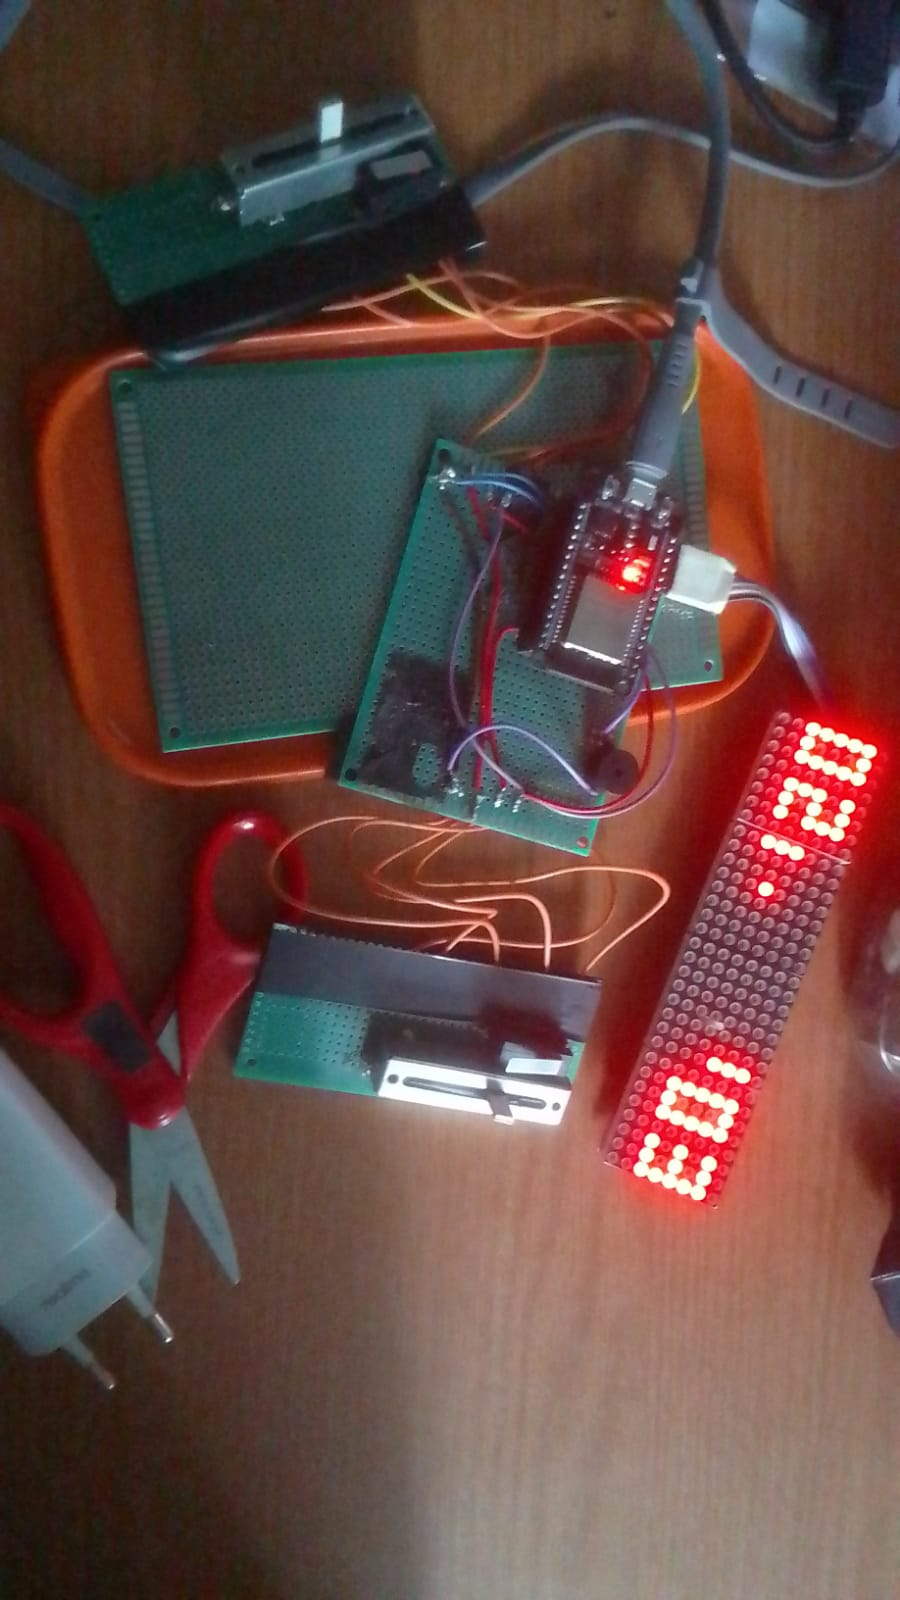
\includegraphics[width=0.5\textwidth]{./images/no-package.jpeg}
    \caption{Hasil tanpa package}
\end{figure}
\end{document}
